\documentclass[tikz,border=10pt]{standalone}

\begin{document}
    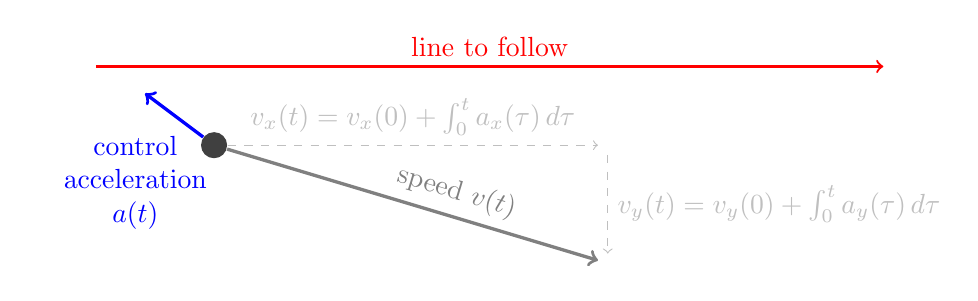
\begin{tikzpicture}
        \draw [thick, red, ->] (0, 0) -- (10, 0) node [pos=0.5,above] {line to follow};
        \node [circle,fill=darkgray,minimum size=1pt] (a) at (1.5, -1) {};
        \node (b) at (6.5, -2.5) {};
        \draw [very thick, gray, ->] (a) -- (b) node [pos=0.6, above, sloped] {speed $v(t)$};
        \node (c) at (6.5, -1) {};
        \draw [lightgray, dashed, ->] (a) -- (c) node [pos=0.5,above] {$v_x(t)=v_x(0) + \int_{0}^{t} a_x(\tau) \,d\tau $};
        \draw [lightgray, dashed, ->] (c) -- (b) node [pos=0.5,right] {$v_y(t)=v_y(0) + \int_{0}^{t} a_y(\tau) \,d\tau $};
        \node (d) at (0.5, -0.25) {};
        \draw [very thick, blue, ->] (a) -- (d) node [yshift=-0.5cm,below,text width=2.5cm,text centered] {control \\ acceleration \\ $a(t)$};
    \end{tikzpicture}
\end{document}